\section{Hard cells and a coupled-target specimen}\label{sec:hard}

\subsection{Structure of a hard cell}
\begin{proposition}[a hard cell is a Minkowski sum of segments]\label{prop:H1}
Let $\Lambda\subseteq\Lambda'$ and let $c=\Pil(u;g_1,\dots,g_j)$ be a hard cell of $U(\Lambda,Q)$ in the sense of \cref{prop:Z}. Put $a_i=-g_i^-\ge0$ and $b_i=g_i^+\ge0$; both lie in $\Lambda'$, have disjoint supports and $g_i=b_i-a_i$. Then $u=\sum a_i$ and
\[
\begin{gathered}c=\sum_i[a_i,b_i]\ \subseteq\ Z^0:=\sum_i\bigl([0,a_i]+[0,b_i]\bigr)\ \subseteq\ [0,Q_c],\\ Q_c=\sum_i(a_i+b_i)\ \text{(the top corner of $c$)}.\end{gathered}
\]
In a fine tiling of $Z^0$ by Graver pieces of the $a_i,b_i$ (\cref{lem:L1,lem:T0}) every tile that does not contain the origin as a vertex is a cell of $U(\Lambda',Q_c)$; the origin is the only vertex that is not a nonzero subset sum. Hence the only part of $c$ that can fail to lie in $U(\Lambda',Q_c)$ is $c\cap\mathrm{St}(0)$, the star of the origin in the tiling.
\end{proposition}
\prov{CW-0503}{E2P4v5-H1}{PROVED}{FULL}
\begin{proof}
$m(c)=u+\sum g_i^-=0$ gives $u=\sum a_i$, and $u+\sum\lambda_ig_i=\sum_i[(1-\lambda_i)a_i+\lambda_ib_i]$, which is a point of $\sum[a_i,b_i]\subseteq Z^0$. The pieces of the $a_i,b_i$ are nonnegative nonzero vectors, so a subset sum vanishes only for the empty subset; the vertices of tiles of $Z^0$ are subset sums and the remaining argument is that of \cref{prop:Z}(Z.1) with $s_i$ the partial sums. Coordinates stay in $[0,Q_c]$ because all pieces are $\ge0$. \qedhere
\end{proof}
This is the precise form of the statement ``the deleted origin matters only for cells that touch every coordinate plane''. In the plane the star of the origin is covered by the coarser rectangular tiling (the proof of \cref{thm:planar}); in the examples of \cref{sec:obstruction} the star of the origin is the corner cube.

\begin{figure}[tbp]\centering
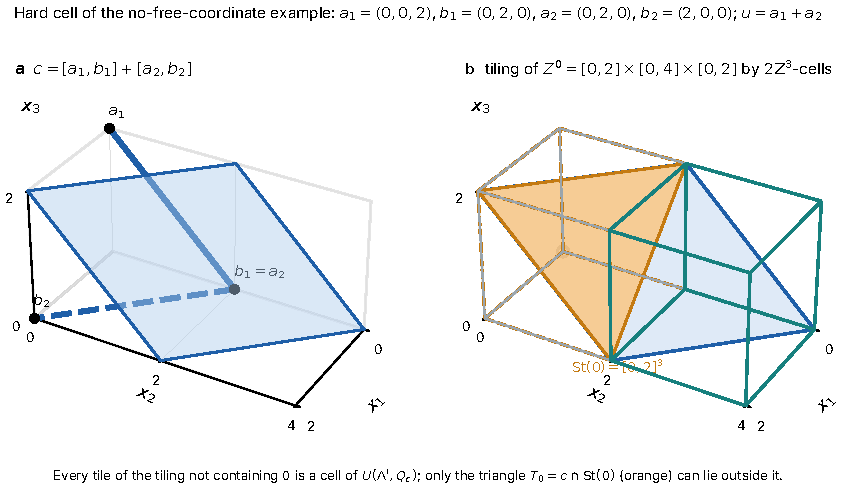
\includegraphics[width=0.98\textwidth]{fig14_hard_cell}
\caption{Minkowski decomposition of a hard cell and the origin star (\cref{prop:H1}; the cell $c$ of \cref{thm:C1}, $\Lambda=2E_3$, $\Lambda'=2\Z^3$; \emph{exact computation}). (a)~$c=[a_1,b_1]+[a_2,b_2]$ with $a_1=(0,0,2)$, $b_1=(0,2,0)$, $a_2=(0,2,0)$, $b_2=(2,0,0)$ and $u=a_1+a_2=(0,2,2)$, drawn as the sum of two segments. (b)~The zonotope $Z^0=[0,2]\times[0,4]\times[0,2]$ tiled by $2\Z^3$-cells: the tile $[0,2]^3$ has the origin as a vertex and is the star $\mathrm{St}(0)$ (orange; it is not a cell of $\Kabs(2\Z^3,Q)$ because the origin is not in the fibre), the tile $[0,2]\times[2,4]\times[0,2]$ is a cell of the target. The only part of $c$ not covered by non-star tiles lies in $\mathrm{St}(0)$; this is the region $T_0$ of \cref{fig:noncontain}.}\label{fig:hardcell}
\end{figure}
\subsection{The coupled specimen P4-F110}
The previous sections concern general lattices. We record the one explicit coupled collective transition for which the whole transport can be decided for every box size $m$.
\begin{proposition}[arithmetic of P4-F110]\label{prop:P4A}
For every integer $m\ge1$, $x_m=2\cdot110^{4m}/9$ has $L=110^{2m}$, $G=9$, $\Cmap(x_m)=110^{4m}/3=:y_m$; the active primes $(2,5,11)$ and the box $Q_m=[0,2m]^3$ are the same for $x_m$ and $y_m$. The relation lattices are $\Lambda_9=\{(a,b,c):a-b+c\equiv0\ (6)\}$ and $\Lambda_3=E_3$, with $\Lambda_9\subsetneq\Lambda_3$; the orders modulo $9$ are $(6,6,6)$ and modulo $3$ are $(2,2,2)$, and both lattices are non-rectangular.
\end{proposition}
\prov{CW-0483}{P4-A}{PROVED}{FULL}
\prov{CW-0484}{P4-L}{PROVED}{FULL}
\begin{proof}
$\mathrm{num}(x_m)=2^{4m+1}5^{4m}11^{4m}$, so $d^2\mid\mathrm{num}$ iff $d=2^a5^b11^c$ with $a,b,c\le2m$. Modulo $9$: $5\equiv2^{-1}$, $11\equiv2$, $\ord_9(2)=6$, so $d\equiv2^{a-b+c}$ and $d\equiv1$ iff $a-b+c\equiv0\ (6)$. Every $d\in D$ has $9\mid d-1$, so $9\mid G$. The vectors $(1,1,0)$ and $(0,1,1)$ give $10,55\in D$ with $\gcd(9,54)=9$, so $G=9$. The vectors $(2m,2m,0)$, $(0,2m,2m)$ give $10^{2m},55^{2m}\in D$, whose lcm is $110^{2m}$, and every $d\in D$ divides $110^{2m}$; so $L=110^{2m}$. Then $\Cmap(x_m)=(2+1)\cdot110^{4m}/9=110^{4m}/3$; the numerator $110^{4m}$ has $v_p=4m$ for $p=2,5,11$, so the primes and the box $[0,2m]^3$ are unchanged. Modulo $3$ all of $2,5,11$ are $-1$, so $\chi_3=(-1)^{a+b+c}$, and $a-b+c\equiv0\ (6)$ implies $a+b+c=(a-b+c)+2b$ even; $(2,0,0)\in E_3\setminus\Lambda_9$. \qedhere
\end{proof}
\begin{theorem}[hull theorem for $E_3$]\label{thm:hull}
Let $n\ge4$ be even and $Q=[0,n]^3$. Then $U(E_3,Q)=\conv F(E_3,Q)=\{z\in[0,n]^3:z_1+z_2+z_3\ge2\}$. For $n=2$ this fails.
\end{theorem}
\prov{CW-0485}{P4-T1}{PROVED}{ADAPTED}
\begin{proof}
(1) \emph{Hull.} $F$ contains all cube vertices except $0$ (their coordinate sums are even) and $(2,0,0),(0,2,0),(0,0,2)$, and every point of $F$ has coordinate sum $\ge2$. The polytope $[0,n]^3\cap\{\sum\ge2\}$ has exactly these $10$ vertices, so $\conv F$ equals it.
(2) \emph{Cube tiling.} $2e_i\in\Gr(E_3)$ (\cref{prop:E25}). For $w\in(2\Z)^3\cap[0,n-2]^3$, $w\ne0$, the eight corners $w+\{0,2\}^3$ have even sum, are nonzero and lie in the box, so the cube is a $3$-cell; these cubes tile $[0,n]^3$ minus the corner cube $[0,2]^3$.
(3) \emph{The corner cube.} We must show $[0,2]^3\cap\{\sum\ge2\}\subseteq U(E_3,[0,n]^3)$. The Graver set of $E_3$ in $[-n,n]^3$ is the same for every $n\ge2$ (a conformally minimal vector lies in the box of its own size) and $F(E_3,4)\subseteq F(E_3,n)$, so the cells of the box-$4$ complex are cells of the box-$n$ complex, and it suffices to take $n=4$. For $n=4$ the argument is a finite exact certificate, identified precisely in \cite{HD1P4}: the object \texttt{n4\_target\_hull\_cover} in \texttt{results/P4\_CERTIFICATES.json} of the release \texttt{GEO\_HD\_E2\_P4\_v001} (byte-identical in \texttt{v001}--\texttt{v004}), replayed by shard \texttt{S4} of that release. It is a decomposition of $\conv F(E_3,[0,4]^3)$ into pieces each lying in a single maximal cell of $\Kabs(E_3,[0,4]^3)$, with no gap nodes; it is a statement about one explicit polytope and one explicit finite set of cells. \emph{Logical role.} The certificate is used for exactly one implication: $[0,2]^3\cap\{\sum x_i\ge2\}\subseteq U(E_3,[0,4]^3)$, from which part~(3) follows for all even $n\ge4$ by the Graver-set argument above. Parts (1) and (2) do not use it. All of \cref{thm:hull}, and everything that cites it (\cref{thm:P4T2,cor:P4C1}), is therefore PROVED \emph{modulo this finite exact computation}, and this status is recorded in \cref{sec:open}. \emph{Independent replay.} Because the certificate is cited and not reproduced, the present manuscript supplies a separate exact check of the same implication (\texttt{scripts/replay\_n4\_cover.py}, output \texttt{results/N4\_COVER\_REPLAY.json}): in exact rational arithmetic it enumerates the $764$ three-dimensional cells of $\Kabs(E_3,[0,4]^3)$ and subtracts them from the polytope $[0,2]^3\cap\{\sum x_i\ge2\}$ by exact polytope subtraction; no piece remains. The same code applied to the box $[0,2]^3$ leaves $9$ pieces, the gap at $n=2$ (the release reports $94$ gap pieces for its own decomposition; piece counts depend on the decomposition used). This replay uses the cells of this manuscript's enumeration and is a manuscript-level check of the implication, not an independent verification of the release. As a further sanity check only, all $609$ points of the quarter-grid of $[0,2]^3$ with coordinate sum $\ge2$ lie in $U(E_3,[0,4]^3)$. For $n=2$ the statement fails: the point $(0,1,\tfrac32)$ lies in $\conv F$ (its sum is $\tfrac52\ge2$) but in no cell of $\Kabs(E_3,[0,2]^3)$ (exact enumeration here; the release certifies the gap at $n=2$ with $94$ gap pieces). This is consistent with the planar face $x_1=0$, where $E_3$ restricts to $E_2$ in the exceptional hollow box $(2,2)$. \qedhere
\end{proof}
\begin{theorem}[transport for P4-F110]\label{thm:P4T2}
For every $m\ge1$: $U(\Lambda_9,Q_m)\subsetneq U(E_3,Q_m)$, the transport class is ``source contained'', and $U(E_3,Q_m)\not\subseteq U(\Lambda_9,Q_m)$.
\end{theorem}
\prov{CW-0486}{P4-T2}{PROVED-SCOPED}{ADAPTED}
\begin{proof}
For $m\ge2$ ($n=2m\ge4$): $U(\Lambda_9)\subseteq\conv F(\Lambda_9)\subseteq\conv F(E_3)=U(E_3)$ by $F(\Lambda_9)\subseteq F(E_3)$ and \cref{thm:hull}. Strictness: $(2,0,0)$ is a vertex of $\conv F(E_3)$ lying in $F(E_3)$ but not in $F(\Lambda_9)$ ($2-0+0=2\not\equiv0\ (6)$); a vertex of $\conv F(E_3)$ that lies in $\conv F(\Lambda_9)\subseteq\conv F(E_3)$ is a vertex of $\conv F(\Lambda_9)$, hence in $F(\Lambda_9)$; so $(2,0,0)\notin U(\Lambda_9)$ (indeed $U(\Lambda_9)\subseteq\conv F(\Lambda_9)$). For $m=1$ ($n=2$, where \cref{thm:hull} fails) the release gives direct exact certificates (the two maximal source cells covered by $18$ target maximal cells, independently replayed); this finite certificate is cited. The reverse non-containment is the same vertex argument. \qedhere
\end{proof}
The scope of the theorem is the family P4-F110 only. A direct engine verification beyond $m=2$ was not attempted by the release (cost); the case $m\ge3$ is covered by \cref{thm:hull}.
\begin{corollary}[predictive criterion for $E_3$ targets]\label{cor:P4C1}
Let $\Lambda\subseteq E_3$ be any sublattice and $n\ge4$ even. Then $U(\Lambda,[0,n]^3)\subseteq U(E_3,[0,n]^3)$.
\end{corollary}
\prov{CW-0489}{P4-C1}{PROVED}{FULL}
\begin{proof}
$U(\Lambda)\subseteq\conv F(\Lambda)\subseteq\conv F(E_3)=U(E_3)$ by \cref{thm:hull}. \qedhere
\end{proof}
The first release of this result added an equality clause (equality of unions iff $\conv F(\Lambda)$ contains the ten vertices of \cref{thm:hull}); that clause is withdrawn (counterexample $\Lambda=2\Z^3$, $n=4$) and only the containment is stated (ER-21).
\prov{CW-0487}{P4-C1 (v001)}{CORRECTED}{EXCLUDED} Its predictive cost is $O(|F|)$ lattice-point tests with no cell reconstruction.
\begin{proposition}[holes are not obstructions; FINITE-EXACT, one specimen]\label{prop:holes}
For $m=1$ the target $E_3$ is not hull-covered (\cref{thm:hull}, $n=2$) and yet $U(\Lambda_9,Q_1)\subseteq U(E_3,Q_1)$.
\end{proposition}
\prov{CW-0488}{P4-O1}{FINITE-EXACT}{FINITE}
This is an observation about one specimen (the release certifies it exactly with $94$ gap pieces); it shows only that gaps of the target do not by themselves obstruct containment.
\begin{figure}[tbp]\centering
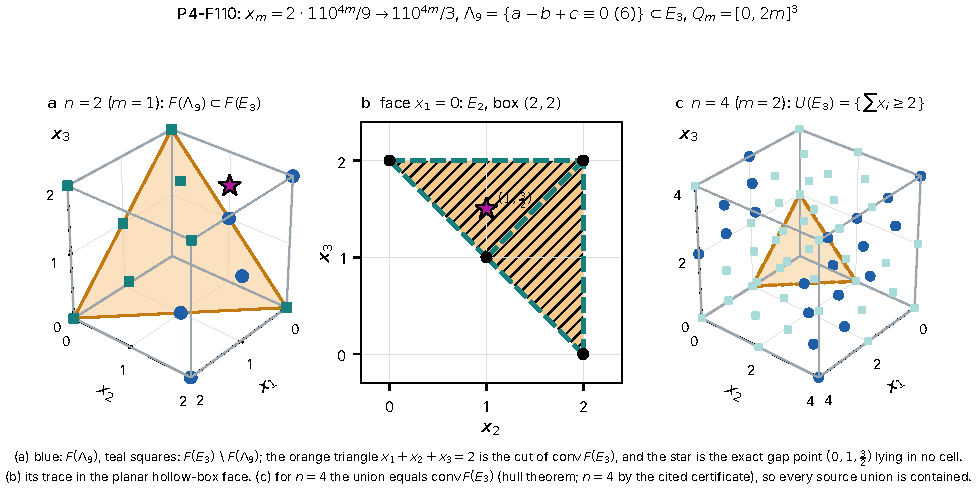
\includegraphics[width=0.98\textwidth]{fig15_f110}
\caption{The coupled family P4-F110 ($x_m=2\cdot110^{4m}/9\to110^{4m}/3$, $\Lambda_9=\{a-b+c\equiv0\ (6)\}\subset E_3$, $Q_m=[0,2m]^3$; \emph{exact computation} for the data, theorem-level for the regime in (c)). (a)~$n=2$ ($m=1$): $F(\Lambda_9,Q_1)$ (5 points) inside $F(E_3,Q_1)$ (13 points); $E_3$ is not hull-covered (\cref{thm:hull}), the point $(0,1,\frac32)$ is in $\conv F(E_3)$ but in no cell of $\Kabs(E_3,Q_1)$. (b)~The face $x_1=0$, where $E_3$ restricts to $E_2$ in the hollow box $(2,2)$ and the gap point appears as $(1,\frac32)$. (c)~$n=4$ ($m=2$): $U(E_3,Q_2)=\{\sum x_i\ge2\}$ by \cref{thm:hull}, with $|F(E_3)|=62$ and $|F(\Lambda_9)|=20$. For $m=1$ containment $U(\Lambda_9)\subseteq U(E_3)$ nevertheless holds (\cref{prop:holes}); for $m\ge2$ it follows from \cref{thm:hull} (see \cref{thm:P4T2}), whose $n=4$ step rests on the certificate of \cref{thm:hull}(3). No claim is drawn from the picture alone.}\label{fig:f110}
\end{figure}
